\section{Inducción}

Principio de Inducción como propiedad de los naturales y técnica para demostraciones matemáticas.
Muy usado en computación además como técnica de construcción de estructuras.

\subsection{Principios de Inducción}
Existen distintas formulaciones para el principio de inducción, veremos las más usadas.

\begin{teorema}[Principio de Buen Orden (PBO).]\label{teo:PBO}
Todo subconjunto no vacío de los naturales tiene un menor elemento\\
\[
\text{si }A\not=\emptyset \text{ y } A\subseteq \N\text{ entonces existe un }x\in A \text{ tal que } x\leq y \text{ para todo }y\in A. 
\]
\end{teorema}

Este principio no lo cumplen por ejemplo los números racionales
>Cuál es el menor elemento del conjunto $A=\{q\in \Q\;|\; q>0\}$? 
No existe un menor elemento, de hecho, supongamos que existiera tal $q_0\in A$ el menor elemento, claramente $\frac{q_0}{2}\in A$ y cumple que $0<\frac{q_0}{2}<q_0$ lo que contradice la hipótesis de que $q_0$ es el menor.
Los reales tampoco cumplen este principio (buen orden).
De hecho el PBO intuitivamente define a $\N$\footnote{En realidad, es un poco más complicado pues el PBO es definitorio para los \emph{ordinales}:
cualquier conjunto que satisface el PBO en general es equivalente a un número ordinal, pero esto escapa un poco de nuestros objetivos.}.

El anterior principio se asume para formular uno más útil:

\begin{teorema}[Principio de Inducción Simple (PIS).]
Sea $A$ un subconjunto de $\N$. Si $A$ cumple con:
\begin{enumerate}
  \item $0\in A$
  \item si $n\in A$ entonces $n+1\in A$
\end{enumerate}
entonces $A=\N$.

\begin{demostracion}
Asumimos el PBO.
Supongamos que tenemos un conjunto $A\subseteq\N$ que cumple las anteriores características y tal que $A\not=\N$.
Entonces el conjunto $B=\N-A$ cumple con $B\subseteq\N$ y con $B\not=\emptyset$.
Por el PBO, $B$ debe tener un menor elemento, digamos $b\in B$.
Es claro que $b\not=0$ (ya que $0\in A$), luego $b-1$ pertenece a $\N$ y no a $B$, por lo que se cumple $b-1\in A$.
Dado que estamos suponiendo que $A$ cumple las características del PIS entonces $b\in A$ lo que contradice el hecho de que $b$ sea el menor elemento de $B$.
La contradicción ocurre por el hecho de suponer que $A\not=\N$, luego necesariamente se cumple que $A=\N$.
\end{demostracion}
\end{teorema}

El anterior principio nos dice que cada vez que nos encontremos con un subconjunto de los naturales que contenga al $0$ y que para cada uno de sus elementos, el sucesor de él también está contenido, entonces el conjunto es exactamente el conjunto de todos los naturales.
Habitualmente a la propiedad $0\in A$ se le llama \emph{base de inducción} (BI), a la suposición de que $n\in A$ se le llama \emph{hipótesis de inducción} (HI), y a la demostración de que $n+1\in A$ se le llama \emph{tésis de inducción} (TI).

¿De qué nos sirve este principio?
Principalmente para demostrar que algunas propiedades son cumplidas por todos los números naturales.

\begin{ejemplo}
Demostraremos que el $0$ es el menor número natural usando el PIS.
Para esto definimos el siguiente conjunto:
\[
A=\{x\in\N\;|\;x\geq 0\}
\]
Si demostramos que $A=\N$ estamos demostrando que para todo elemento $x\in\N$, $x$ es mayor o igual a $0$ y que por lo tanto $0$ es el menor natural.

\begin{demostracion}
La demostración es bastante simple:
\begin{inducciondemo}
\BI Claramente $0\in A$ ya que $0\geq 0$.
\HI Supongamos que un natural $n$ fijo cumple con $n\geq 0$.
\TI Dado que $n\geq 0$ se cumple que $n+1\geq 1$ y por lo tanto $n+1\geq 0$
\end{inducciondemo}
Por PIS se sigue que $A=\N$.
\end{demostracion}
\end{ejemplo}

Generalmente el PIS se formula de una manera alternativa que hace más fácil plantear ciertos teoremas:

\begin{teorema}[Principio de Inducción Simple (segunda formulación).]
Sea $P$ una propiedad cualquiera sobre elementos de $\N$.
Si se tiene que:
\begin{enumerate}
\item $P(0)$ es verdadero ($0$ cumple la propiedad $P$)
\item $P(n)\Rightarrow P(n+1)$ (cada vez que $n$ cumple la propiedad $n+1$ también la cumple)
\end{enumerate}
Entonces todos los elementos de $\N$ cumplen la propiedad $P$.

\begin{demostracion}
La demostración es inmediata a partir de la primera formulación del PIS, sólo tome $A=\{n\in\N\;|\; P(n)$ es verdadera $\}$.
\end{demostracion}
\end{teorema}

Al igual que en la formulación anterior, a $P(0)$ se le llama BI, la suposición de $P(n)$ es HI, y la demostración de $P(n+1)$ a partir de $P(n)$ es la TI. 

\begin{ejemplo}
Demostraremos que la siguiente propiedad se cumple para todo $n$:
\[
\sum_{i=0}^{n}i=\frac{n(n+1)}{2}
\]
Para ocupar el PIS debemos definir nuestra propiedad $P$, en este caso:
\[
P(n)\;:\; \sum_{i=0}^{n}i=\frac{n(n+1)}{2}
\]

\begin{demostracion}
\begin{inducciondemo}
\BI Si $n=0$, $\sum_{i=0}^{n}=\sum_{i=0}^{0}=0$ que es igual a $\frac{n(n-1)}{2}=0$, por lo que $P(0)$ es verdadera
\HI Supongamos que $P(n)$ se cumple, o sea que $\sum_{i=0}^{n}i=\frac{n(n-1)}{2}$
\TI Queremos demostrar ahora que $P(n+1)$ se sigue cumpliendo, o sea, queremos demostrar que
\[
P(n+1)\;:\; \sum_{i=0}^{n+1}i=\frac{(n+1)((n+1)+1)}{2}
\]
es verdadero.

Ahora, es claro que
\[
\sum_{i=0}^{n+1}i=(\sum_{i=0}^{n}i)+(n+1)
\]
Por HI se cumple que
\[
\sum_{i=0}^{n+1}i=(\frac{n(n+1)}{2})+(n+1)
\]
de lo que resulta 
\[
\sum_{i=0}^{n+1}i=\frac{(n^2+n+2n+2)}{2}=\frac{n^2+3n+2}{2}=\frac{(n+1)(n+2)}{2}
\]
finalmente
\[
\sum_{i=0}^{n+1}i=\frac{(n+1)((n+1)+1)}{2}
\]
por lo que $P(n+1)$ es también verdadero.
\end{inducciondemo}
Por PIS se sigue que $P$ se cumple para todos los naturales.
\end{demostracion}
\end{ejemplo}

A veces necesitamos demostrar propiedades que se cumplen para todos los naturales exceptuando una cantidad finita de ellos.
Generalmente son propiedades de los naturales que empiezan a cumplirse desde un punto en adelante.
El PIS puede ser modificado para que la BI pueda iniciarse en cualquier número natural distinto de $0$, lo que nos importa en estos casos es que cierta propiedad se cumple para todos los naturales mayores o iguales que cierto natural fijo.
Debemos cambiar entonces la demostración de nuestra base a ese natural fijo.
El siguiente ejemplo nos muestra una aplicación de esta variación del PIS.

\begin{ejemplo}
Para todo natural $n\geq 4$ se cumple que 
\[
n!>2^n
\]
Nuestra propiedad en este caso es $P(n)\;:\;n!>2^n$.

\begin{demostracion}
\begin{inducciondemo}
\BI En este caso la base debiera iniciarse en $n=4$, entonces nos preguntamos si $P(4)$ es o no verdadero.
Ahora, $4!=1\cdot 2\cdot 3\cdot 4=24>16=2^4$, por lo que la propiedad se cumple para $4$.
\HI Supongamos que efectivamente $n!>2^n$
\TI Queremos demostrar que $(n+1)!>2^{n+1}$.
Ahora, 
\[
(n+1)!=(n+1)n!
\]
dado que estamos suponiendo que $n$ cumple la propiedad (HI) tenemos que
\[
(n+1)!=(n+1)n!>(n+1)2^n
\]
Ahora, dado que la propiedad que queremos demostrar se inicia en $n=4$ sabemos que $n+1$ es necesariamente mayor que $4$ por lo que obtenemos
\[
(n+1)!>(n+1)2^n>4\cdot 2^n>2\cdot 2^n=2^{n+1}
\]
de donde obtenemos que
\[
(n+1)!>2^{n+1}
\]
por lo que la propiedad se cumple también para $n+1$.
\end{inducciondemo}
\end{demostracion}
\end{ejemplo}

¿Cómo podemos justificar este nuevo uso del PIS a partir de la formulación con base en 0?
En vez de considerar la propiedad $P$ de arriba, pordiamos considerar la propiedad:
\[
n<4 \text{ o }n!>2^n.
\]
note que esta propiedad es verdadera (se puede demostrar usando PIS) para todos los elementos de $\N$.

Existen casos donde la inducción sirve para problemas que parecen estar muy apartados de propiedades numéricas como en el siguiente ejemplo:

\begin{ejemplo}
Queremos demostrar que cualquier tablero cuadriculado de dimensiones $2^n\times 2^n$ con $n\geq 1$ al que le falta exactamente un casillero, puede ser cubierto completamente con \emph{trominós}.
Un \emph{trominó} es una ficha como la que se muestra en la figura~\ref{fig:tromino}.

\begin{figure}[h!]
\begin{center}
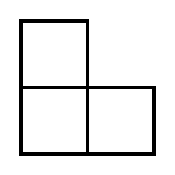
\includegraphics{eps_imgs/tromino.eps}
\end{center}
\caption{Un \emph{trominó} recto}
\label{fig:tromino}
\end{figure}

La propiedad en este caso tiene que ver con la potencia que nos da las dimensiones del tablero, o sea $P$ sería:
\begin{center}
$P(n)\;:\;$ un tablero de $2^n\times 2^n$ con un casillero menos, puede ser completamente cubierto con \emph{trominós}.
\end{center}
Lo segundo que debemos observar es que en este caso la inducción comienza en $n=1$.

\begin{demostracion}
(Demostración en clases)
\end{demostracion}
\end{ejemplo}

Al alumno de computación el anterior ejemplo debiera de inmediato parecerle, además de una demostración, un método de construcción.
Usando exactamente la misma idea de la anterior demostración se podría programar un algoritmo recursivo que, dado un tablero de dimensiones $2^n\times 2^n$ al que le falta un casillero, pueda encontrar (efectivamente) una forma de cubrirlo usando \emph{trominós}.

Existe una tercera formulación del Principio de Inducción que usa una suposición más fuerte y resulta de gran utilidad para demostrar propiedades cuando la información de que $n$ cumple la propiedad no basta para concluir que $n+1$ también la cumple.

\begin{teorema}[Principio de Inducción por Curso de Valores (PICV).]
Sea $A$ un subconjunto de $\N$.
Si para todo $n\in\N$ se cumple que 
\[
si \{x\in \N\mid x<n\} \subseteq A \text{ entonces } n\in A,
\]
entonces $A=\N$.
\end{teorema}
En este caso la parte $\{0,1,\ldots,n-1\}\subseteq A$ es la HI, y la demostración de $n\in A$ es la TI.
Un punto interesante es que \emph{pareciera} no haber una base de inducción... (¿la hay? piense en el caso $\emptyset\subseteq A$).

Al igual que con el PIS, existe una segunda formulación que hace las demostraciones más naturales.

\begin{teorema}[Principio de Inducción por Curso de Valores (segunda formulación).]
Sea $P$ una propiedad cualquiera sobre elementos de $\N$ y suponga que se cumple que:
\[
\text{si para todo }k\in\N\text{ menor que }n\text{ }P(k)\text{ es verdadero, entonces }P(n)\text{ es verdadero}.
\]
Entonces se tiene que $P$ es verdadero para todos los elementos de $\N$.
\end{teorema}

El teorema anterior nos dice que si, al suponer que cierta propiedad se cumple para todos los números naturales menores que cierto $n$ podemos concluir que $n$ también la cumple, entonces se concluye que todos los números naturales cumplen la propiedad.

\begin{ejemplo}
La sucesión de Fibonacci, es una serie de números naturales $F_0,F_1,F_2,\ldots,F_n,F_{n+1}\ldots$ que cumplen la siguiente relación de recurrencia:
\[
\begin{array}{rcl}
F_0 & = & 0 \\
F_1 & = & 1 \\
F_n & = & F_{n-1} + F_{n-2} \;\;\;\forall n\geq 2
\end{array}
\]
Demostraremos que $F_n<2^n$ para todo $n\in\N$.

\begin{demostracion}
La demostración la haremos usando el PICV.
Un punto interesante es que usaremos dos casos base, $n=0$ y $n=1$, la razón debiera quedar clara cuando finalizemos la demostración.
\begin{inducciondemo}
\BI Para $n=0$ se tiene $0<1=2^0$, para $n=1$ se tiene que $1<2=2^1$ por lo que los casos base funcionan.
\HI Supongamos que para todo $k<n$ se cumple que $F_k<2^k$.
\TI Queremos demostrar que usando HI podemos concluir que $F_n<2^n$.
Usaremos el hecho de que $F_n=F_{n-1}+F_{n-2}$, y la HI:
\[
\begin{array}{rcl}
F_n & = & F_{n-1} + F_{n-2} \\
 & \stackrel{\text{(HI)}}{<} & 2^{n-1}+2^{n-2} = \frac{3}{4}\cdot 2^n \\
 & < & 2^n \\
\end{array}
\]
\end{inducciondemo}
Por el PICV se sigue que $F_n<2^n$ para todo $n\in\N$.
\end{demostracion}
\end{ejemplo}

Un error muy frecuente entre los alumnos es hacer la inducción ``al revés''.
Inicialmente suponen que la tesis de inducción es correcta y haciendo movimientos algebráicos obtiene la hipótesis de inducción con lo que dan por terminada su demostración.
Este tipo de desarrollo se considerará siempre incorrecto ya que {\bf no se puede partir una demostración desde lo que se quiere concluir}.
Siempre se debe tener muy en claro que lo que debemos suponer es la hipótesis de inducción y a partir de ella concluir la tesis de inducción.

Más adelante en el curso veremos aplicaciones directas de los principios de inducción en el área de algoritmos computacionales, principalmente en el cálculo de la eficiencia de un algoritmo y en el establecimiento de su corrección (que el algoritmo efectivamente hace lo que dice que hace).

\subsection{Inducción Estructural}
Hemos visto distintos principios de inducción (y formulaciones de estos), todos aplicados al conjunto de los números naturales.
¿Qué tiene de especial $\N$?
Principalmente su característica de ser un conjunto que se puede construir a partir de un elemento base y un operador.
El elemento base es el $0$ y el operador es ``el sucesor''.
Intuitivamente todo natural se puede obtener a partir de sumarle $1$ a otro natural, o sea de aplicarle el operador sucesor a otro natural (excepto el $0$ que es la base).
Así una forma de definir al conjunto de los números naturales es la siguiente:
\begin{enumerate}
\itemsep 0pt
\item El $0$ es un número natural.
\item Si $n$ es un número natural entonces $n+1$ también es un número natural.
\item Todos los números naturales y sólo ellos se obtienen a partir de la aplicación de reglas 1 y 2.
\end{enumerate}
Mirando la definición debiera quedar clara la naturaleza constructiva de los números naturales y como se relaciona con el principio de inducción.
Lo que hacemos entonces para demostrar que una propiedad se cumple para todo el conjunto de los números naturales es demostrar que se cumple para su elemento base y que si suponemos que se cumple para un elemento cualquiera, el operador de construcción (sucesor en este caso) mantiene la propiedad.

¿Pueden otros conjuntos definirse de manera similar?
La respuesta es afirmativa y a estas definiciones les llamaremos \emph{definiciones inductivas}.
La implicancia más importante es que podremos usar inducción para demostrar propiedades que cumplen otros conjuntos, no sólo los naturales.
Una implicancia adicional es que podremos definir nuevos objetos (funciones, operaciones, etc) usando la definición inductiva del conjunto.

En general para definir un conjunto inductivamente necesitaremos:
\begin{enumerate}
\itemsep 0pt
\item Un conjunto (no necesariamente finito) de elementos base que se supondrá que inicialmente pertenecen al conjunto que queremos definir.
\item Un conjunto finito de reglas de construcción de nuevos elementos del conjunto a partir de elementos que ya pertenecen.
\end{enumerate}
(Omitiremos la afirmación ``Todos los elementos del conjunto y sólo ellos se obtienen a partir de la aplicación de las anteriores reglas'' pero supondremos que está implícita en la definición.)

\begin{ejemplo}
Un ejemplo muy sencillo es la definición de los números pares.
\begin{enumerate}
\itemsep 0pt
\item El $0$ es un número par.
\item Si $n$ es un número par entonces $n+2$ es un número par.
\end{enumerate}
nada muy extraño...
\end{ejemplo}

Un punto muy importante es que ningún elemento del conjunto que queremos definir se debe escapar de nuestra definición, por ejemplo la siguiente {\bf no} es una definición válida de los números pares:
\begin{enumerate}
\itemsep 0pt
\item El $0$ es un número par.
\item Si $n$ es un número par entonces $2n$ es un número par.
\end{enumerate}
¿Cuál es el problema?...

\begin{ejemplo}
Muchas veces cuando estudiamos computación nos encontramos con estructuras de datos.
Generalmente las usamos y no nos interesa demasiado formalizar ni su construcción ni las operaciones sobre ella.
En este ejemplo veremos como podemos formalizar un concepto similar al de ``lista enlazada'' muy usada en cursos de computación. 
Para simplificar la definición, supondremos que nuestras listas sólo pueden contener números naturales.

Un ejemplo de lista enlazada (de las que usaremos nosotros) es:
\[
\rightarrow 5\rightarrow 7\rightarrow 1\rightarrow 0\rightarrow 3\rightarrow 1\rightarrow 4
\]
Diremos en este caso que la lista contiene a los valores $5, 7, 1, 0, 3, 1, 4$ en ese orden (note la repetición del elemento $1$).
Una lista muy especial es la lista vacía que representaremos por
\[
\emptyset
\]
que es una lista que no contiene elemento alguno (para los que son más orientados a la programación esta lista representaría a un puntero nulo, \texttt{NULL} en C).
En este caso la lista
\[
\emptyset\rightarrow 10\rightarrow 6
\]
y la lista
\[
\rightarrow 10\rightarrow 6
\]
son exactamente iguales, ambas contienen exactamente a los elementos $10$ y $6$ en ese orden.

Con estas consideraciones no es difícil imaginar que cualquier lista que se nos ocurra se formará a partir de una lista más pequeña a la que se le ha agregado un elemento ``al final''.
La única lista que no puede ser creada entonces de esta manera es la lista vacía, que debiera ser nuestro caso base.
Así la siguiente es una definición para el conjunto $\L_\N$ de todas las listas formadas con elementos en $\N$.
\begin{enumerate}
\itemsep 0pt
\item $\emptyset$ es una lista y representa a la lista vacía ($\emptyset\in\L_\N$).
\item Si $L$ es una lista y $k$ es un natural, entonces $L\rightarrow k$ es una lista ($L\in\L_\N\Rightarrow L\rightarrow k\,\in\L_\N,\;\forall k\in\N$).
\end{enumerate}

En este caso la ``operación'' que estamos usando para crear listas es tomar una lista, y agregar una flecha ($\rightarrow$) seguida de un natural.
La ``operación flecha seguida de natural'' correspondería a sumar uno en el caso de la inducción sobre los naturales.
La anterior definición nos dice que $\emptyset$ es una lista, que $\rightarrow 4$ es una lista ya que se forma a partir de la lista vacía $\emptyset$ agregándole el natural $4$.
De la misma forma $\rightarrow 4\rightarrow 7$ es una lista ya que se forma a partir de $\rightarrow 4$ que sabemos que es una lista, al agregar el natural $7$.

Esta anterior definición además nos entrega una noción de igualdad de listas (concepto muy importante en los ejemplos posteriores):
\[
L_1\rightarrow k = L_2\rightarrow j \;\;\text{ si y sólo si }\;\; L_1=L_2 \text{ y } k=j
\]
esto quiere decir que dos listas son iguales cuando ambas han sido creadas a partir de la misma lista agregándole el mismo elmento al final.

Podemos plantear algunas propiedades que debieran cumplir todas las listas y demostrarlas por inducción estructural, es decir usando inducción en el dominio constructible de las listas.
Demostraremos a modo de ejemplo que toda lista tiene exactamente la misma cantidad de elementos que de flechas ($\rightarrow$).

\begin{demostracion}
En este caso la propiedad $P$ es sobre el conjunto $\L_\N$ de todas las listas con elementos naturales y se define por:
\[
P(L)\;:\;L\text{ tiene el mismo número de flechas que de elementos.}
\]
\begin{inducciondemo}
\BI El caso base es la lista vacía, ella tiene ningún elemento y ninguna flecha por lo que cumple con la propiedad, o sea $P(\emptyset)$ es verdadero.
\HI Supongamos que una lista cualquiera $L$ tiene exactamente tantos elementos como flechas, o sea que $P(L)$ es verdadero.
\TI Queremos demostrar que $P(L\rightarrow k)$ es verdadero, o sea que la lista $L\rightarrow k$ con $k\in\N$, también cumple la propiedad.
%\footnote{note que en este caso decir $L\rightarrow  k$ es equivalente a decir $n+1$ en el PIS.}
Es claro que la lista $L\rightarrow k$ tiene exactamente una flecha más y exactamente un elemento más que $L$.
Dado que estamos suponiendo que $P(L)$ se cumple (HI), concluimos que $L\rightarrow k$ tiene exactamente el mismo número de flechas que de elementos, por lo que $P(L\rightarrow k)$ también se cumple.
\end{inducciondemo}
Por inducción estructural se sigue que todas las listas en $\L_\N$ tienen la misma cantidad de flechas que de elementos.
\end{demostracion}
\end{ejemplo}

Algo muy interesante de las definiciones inductivas de conjuntos, es la posibilidad de aprovechar el carácter de constructivo para definir operadores o funciones sobre los elementos.
Cuando estas definiciones se hacen en los naturales generalmente se les llama ``definiciones recursivas'', por ejemplo, la definición del operador factorial ($!$) sobre $\N$ se hace de la siguiente manera:
\begin{enumerate}
\itemsep 0pt
\item $0!=1$.
\item $(n+1)!=(n+1)\cdot n!$.
\end{enumerate}
Aquí se está aprovechando la forma de construcción de los naturales para definir de manera elegante un operador sobre todos los naturales.
Se define el caso base ($0$) y se explicita como operar el siguiente elemento que ha sido creado por inducción (sucesor) suponiendo que el operador ya está definido sobre los demás elementos del conjunto.

De manera similar podemos definir funciones y operadores sobre otros conjuntos creados por inducción estructural, el siguiente ejemplo muestra definiciones para el dominio de las listas.

\begin{ejemplo}
La función $|\cdot|:\L_\N\rightarrow\N$ (que a la lista $L$ se aplica como $|L|$) toma una lista como argumento y entrega el entero correspondiente a la cantidad de elementos de la lista, es decir el largo de la lista.
Queremos definir la función $|\cdot|$ inductivamente sobre el dominio constructible de las listas $\L_\N$.
Primero debemos definir el caso base, o sea el resultado de $|\emptyset|$.
Naturalmente el resultado debiera ser $0$, luego la primera parte de nuestra definición debiera ser:
\[
|\emptyset| = 0
\]
Queremos definir ahora que pasa con el largo de una lista que ha sido creada a partir de otra anterior.
La única forma que conocemos de crear una nueva lista es agregarle un elemento al final de la primera, es claro que el largo de la nueva lista será el largo de la primera más 1, luego la segunda parte de nuestra definición debiera ser:
\[
|L\rightarrow k|=|L|+1
\]

Finalmente la definición completa de la función $|\cdot|$ que toma una lista y entrega su largo resulta:
\begin{enumerate}
\itemsep 0pt
\item $|\emptyset|=0$
\item $|L\rightarrow k|=|L|+1$
\end{enumerate}
con $L$ lista y $k\in\N$.
\end{ejemplo}

La noción de largo de una lista ya la habíamos usamos, de manera intuitiva, cuando demostramos que toda lista tiene exactamente la misma cantidad de flechas que de elementos.
De la misma forma como definimos $|\cdot|$ podríamos definir la función $\stackrel{\rightarrow}{|\cdot|}:\L_\N\rightarrow\N$ que toma una lista cualquiera y entrega como resultado la cantidad de flechas de la lista.
Así la demostración de que toda lista tiene exactamente la misma cantidad de flechas que de elementos puede formularse como:
\[
\forall L\in\L_\N\;\;\;\stackrel{\rightarrow}{|L|}=|L|
\]
Más adelante veremos propiedades de las listas que tienen que ver con funciones y operadores definidos para ellas y que pueden demostrarse por inducción.

\begin{ejemplo}
La función $\text{sum}:\L_\N\rightarrow\N$ toma una lista como argumento y entrega el entero correspondiente a la suma de todos los elementos de la lista.
Por ejemplo
\[
\text{sum}(\rightarrow 5\rightarrow 7\rightarrow 1\rightarrow 0\rightarrow 3\rightarrow 1\rightarrow 4)=21
\]
Definiremos la función $\text{sum}$ de forma inductiva sobre el dominio constructible de las listas.
Primero debemos definir el caso base, o sea el resultado de aplicar $\text{sum}$ a la lista vacía.
Naturalmente el resultado debiera ser $0$, ya que la lista no contiene elemento alguno.
Ahora tenemos que arreglárnosla para definir $\text{sum}$ para una lista cualquiera construida a partir de una lista anterior.
Es claro que sumar todos los elementos de una lista es equivalente a sumar todos los elementos del tramo inicial de la lista y al resultado sumarle el último elemento.
Finalmente la definición completa de la función $\text{sum}$ que toma una lista y entrega la suma de sus valores resulta:
\begin{enumerate}
\itemsep 0pt
\item $\text{sum}(\emptyset)=0$
\item $\text{sum}(L\rightarrow k)=\text{sum}(L)+k$
\end{enumerate}
con $L$ lista y $k\in\N$.

Usando esta definición podemos calcular la suma de la lista $\rightarrow 2\rightarrow 3\rightarrow 5$ de la siguiente manera:
\[
\begin{array}{rcl}
\text{sum}(\rightarrow 2\rightarrow 3\rightarrow 5) & = & \text{sum}(\rightarrow 2\rightarrow 3) + 5 \\
& = & \text{sum}(\rightarrow 2) + 3 + 5\\
& = & \text{sum}(\emptyset) + 2 + 3 + 5\\
& = & 0 + 2+ 3 + 5\\
& = & 10
\end{array}
\]
\end{ejemplo}

\begin{ejemplo}
Definiremos la función $\max:\L_\N\rightarrow\N\cup\{-1\}$ de una lista, que entrega el valor del elemento más grande en la lista.
Por convención, supondremos que el elemento máximo de la lista vacía es $-1$ (¿Por qué tiene sentido esta suposición?).
Nuestra definición entonces resulta:
\begin{enumerate}
\itemsep 0pt
\item $\max(\emptyset)=-1$
\item $
\max(L\rightarrow k)=\left\{
\begin{array}{cl}
\max(L) & \text{si }\max(L)\geq k \\
k & \text{si }k>\max(L)
\end{array}\right.
$
\end{enumerate}
Como ejercicio se puede hacer algo similar al ejemplo anterior para calcular $\max(\rightarrow 4\rightarrow 1\rightarrow 7\rightarrow 3)$.
\end{ejemplo}

\begin{ejemplo}
En este ejemplo veremos la definición de la función $Head:\L_\N\rightarrow\N$ que dada una lista entrega el primer elemento contenido en ella (la ``cabeza'' de la lista).
Una cosa interesante de esta función es que no está definida para todas las listas de naturales, de hecho la lista vacía no tiene elemento alguno, por lo tanto no tiene un primer elemento.
La función estará entonces, parcialmente definida por inducción.
\begin{enumerate}
\itemsep 0pt
\item $Head(\rightarrow k)=k$
\item Si $L$ es una lista no vacía $(L\not=\emptyset)$, $Head(L\rightarrow k)=Head(L)$.
\end{enumerate}
Se debe notar que para esta definición existe una infinidad de casos base (tantos como elementos de $\N$).
\end{ejemplo}

Todos los anteriores ejemplos tienen que ver con funciones sobre listas que entregan un elemento natural, en la siguiente definición veremos un operador sobre listas, es decir, una función que toma una lista y entrega como resultado otra lista.

\begin{ejemplo}
Queremos definir el operador $Suf:\L_\N\rightarrow\L_\N$ (operador \emph{sufijo}) que toma una lista y entrega la lista que resulta de ella al sacar el primer elemento.
La definición entonces resulta:
\begin{enumerate}
\itemsep 0pt
\item $Suf(\rightarrow k)=\emptyset$
\item Si $L$ es una lista no vacía, $Suf(L\rightarrow k)=Suf(L)\rightarrow k$.
\end{enumerate}
Note que en este caso el operador tampoco está definido para la lista vacía.
\end{ejemplo}

Ahora con las varias funciones definidas podemos plantear muchas propiedades acerca de listas y demostrarlas usando inducción estructural.

\begin{teorema}
Las siguientes son propiedades de las listas:
\begin{enumerate}
\itemsep 0pt
\item $\forall L\in\L_\N$ se cumple $\text{sum}(L)\geq 0$.
\item $\forall L\in\L_\N$ se cumple $\max(L)\leq\text{sum}(L)$. \label{listprop1}
%\item $\forall L\in\L_\N$, $L\not=\emptyset$ se cumple que $L=\rightarrow Head(L)Suf(L)$.
\item $\forall L\in\L_\N$, $\text{sum}(L)=Head(L)+\text{sum}(Suf(L))$.
\item $\forall L_1,L_2\in\L_\N$, $L_1,L_2\not=\emptyset$, se cumple $L_1=L_2$ si y sólo si $Suf(L_1)=Suf(L_2)$ y $\text{sum}(L_1)=\text{sum}(L_2)$. \label{listprop2}
\item Muchas otras propiedades que se pueden plantear...
\end{enumerate}
\begin{demostracion}
A modo de ejemplo demostraremos sólo las propiedades~\ref{listprop1} y~\ref{listprop2}, las demás se proponen como ejercicios.
\begin{enumerate}
	\setcounter{enumi}{1}
	\item Por inducción estructural en $\L_\N$:
	\begin{inducciondemo}
		\BI $\max(\emptyset)=-1\leq 0=\text{sum}(\emptyset)$, por lo que $\emptyset$ cumple la propiedad.
		\HI Supongamos que para toda lista $L$ se cumple que $\max(L)\leq\text{sum}(L)$.
		\TI Queremos demostrar que $L\rightarrow k$ con $k\in \N$ también cumple, o sea, $\max(L\rightarrow k)\leq\text{sum}(L\rightarrow k)$.
		
		La definición de la función $\max$ nos habla de dos casos
		\[
		\max(L\rightarrow k)=\left\{
		\begin{array}{cl}
		\max(L) & \text{si }\max(L)\geq k \\
		k & \text{si }k>\max(L)
		\end{array}\right.
		\]
		seguiremos la demostración para cada uno de estos casos:
		
		Si $\max(L\rightarrow k)=\max(L)$ tenemos que
		  \[
		  \begin{array}{rcl}
		  \max(L\rightarrow k) & = & \max(L) \\
		  & \leq & \max(L) + k \;\;\; \text{(ya que }k\in\N\text{)}\\
		  & \stackrel{\text{HI}}{\leq}& \text{sum}(L) + k \; =\; \text{sum}(L\rightarrow k)
		  \end{array}
		  \]
		
		Si $\max(L\rightarrow k)=k$ tenemos que
		  \[
		  \max(L\rightarrow k)\;\;=\;\;k\;\stackrel{\text{(1.)}}{\leq}\;\;\text{sum}(L) + k\;\;=\;\;\text{sum}(L\rightarrow k)
		  \]
		
		En cualquier caso se cumple que $\max(L\rightarrow k)\leq\text{sum}(L\rightarrow k)$, luego por inducción estructural se sigue que la propiedad se cumple para todas las listas.
	\end{inducciondemo}
	\setcounter{enumi}{3}
	\item Primero, es claro que si $L_1=L_2$ entonces se cumple que $Suf(L_1)=Suf(L_2)$ y que $\text{sum}(L_1)=\text{sum}(L_2)$ ya que ambas son funciones y la igualdad está bien definida.
	El punto complicado es demostrar la implicación inversa: si $Suf(L_1)=Suf(L_2)$ y $\text{sum}(L_1)=\text{sum}(L_2)$ entonces $L_1=L_2$.
	Demostraremos esto útlimo por inducción estructural en $\L_\N$:
	\begin{inducciondemo}
	  \BI En este caso no podemos tomar $\emptyset$ como base ya que $Suf$ no está definido para $\emptyset$.
	  Tomaremos como base entonces listas con un elemento.
	  Sean $L_1=\rightarrow k$ y $L_2=\rightarrow j$ dos listas, dado que $\text{sum}(L_1)=\text{sum}(L_2)$ tenemos que $\text{sum}(\rightarrow k)=\text{sum}(\rightarrow j)$ y por lo tanto $k=j$ por lo que las listas $L_1$ y $L_2$ son iguales.
	  \HI Supongamos que si $Suf(L_1)=Suf(L_2)$ y $\text{sum}(L_1)=\text{sum}(L_2)$ entonces $L_1=L_2$ para cualquier par de listas $L_1$, $L_2$.
	  \TI Sean ahora dos listas $L_1\rightarrow k$ y $L_2\rightarrow j$, tales que
	  \[
	  \begin{array}{l}
	  Suf(L_1\rightarrow k)=Suf(L_2\rightarrow j) \;\;\;\text{ y} \\
	  \text{sum}(L_1\rightarrow k)=\text{sum}(L_2\rightarrow j)\text{.}
	  \end{array}
	  \]
	  Por la definición de $Suf$ y $\text{sum}$ obtenemos 
	  \[
	  \begin{array}{l}
	  Suf(L_1)\rightarrow k = Suf(L_2)\rightarrow j \\
	  \text{sum}(L_1)+k=\text{sum}(L_2)+j
	  \end{array}
	  \]
	  de la primera de estas ecuaciones y usando la definición de igualdad de listas obtenemos el hecho de que necesariamente $Suf(L_1)=Suf(L_2)$ y que $k=j$.
	  Usando este último resultado en la segunda ecuación obtenemos que $\text{sum}(L_1)=\text{sum}(L_2)$.
	  Tenemos entonces que $Suf(L_1)=Suf(L_2)$, $\text{sum}(L_1)=\text{sum}(L_2)$, y por la HI resulta que $L_1=L_2$ y dado que $k=j$ obtenemos que $L_1\rightarrow k=L_2\rightarrow j$.
	\end{inducciondemo}
	%Por inducción estructural sobre $\L_\N$ se cumple que para todo par de listas no vacías la propiedad se cumple.
\end{enumerate}
\end{demostracion}
\end{teorema}

Los ejemplos anteriores tienen que ver con la construcción de listas.
Un punto que se debe notar es que cada lista se construye a partir de una única lista anterior, al igual que en el PIS en donde el paso inductivo tiene que ver exclusivamente con el antecesor de un natural.
De manera similar al PICV podemos definir conjuntos inductivamente, usando para la construcción de un elemento particular uno o más de los elementos anteriores (anteriormente construidos).
Luego para definir propiedades y demostrar teoremas sobre el nuevo conjunto definido tendremos que usar una estrategia más similar al PICV que al PIS.
En el siguiente ejemplo veremos como se aplican estas ideas.

\begin{ejemplo}
Queremos definir el conjunto $\E_{\N}$ de todas las expresiones aritméticas que se pueden formar con números naturales, el símbolo \texttt{+}, el símbolo \texttt{*} y los símbolos de paréntesis \texttt{(} y \texttt{)}.
	Por ejemplo, los siguientes son elementos de $\E_{\N}$ (son expresiones aritméticas)
	\begin{center}
	\texttt{( $4$ + $5$ * $7$ ) * $9$} \\
	\texttt{$12$ + $2$ + $3$ + $2$ * $11$} \\
	\texttt{( $143$ + $9$ )} \\
	\texttt{$3$}
	\end{center}
	Note que no nos interesa el \emph{valor} de la expresión, sólo nos interesa la forma en que esta ``se ve''.
	El conjunto $\E_\N$ puede definirse inductivamente usando una definición inductiva por curso de valores, es decir, definiendo un elemento posiblemente a partir de varios de los elementos anteriores.
	Una expresión vacía no tiene sentido, así que nuestro caso base (la expresión más pequeña) sería un natural cualquiera, luego:
	\begin{center}
	Si $k$ es un natural, entonces $k$ es una expresión ($k\in\N\;\Rightarrow\;k\in\E_\N$).
	\end{center}
	No es difícil notar que otra manera de crear una expresión es ``sumando'' dos expresiones, o más formalmente, poniéndole un símbolo \texttt{+} entre las expresiones, así uno de los pasos inductivos será:
	\begin{center}
	Si $E_1$ y $E_2$ son expresiones, entonces \texttt{$E_1$ + $E_2$} es una expresión (\texttt{$E_1,E_2\in\E_\N\;\Rightarrow\;E_1$ + $E_2\in\E_\N$}).
	\end{center}
	Necesitamos completar la definición inductiva de las expresiones aritméticas, especificando como crear expresiones usando \texttt{*} y \texttt{()}.
	Finalmente nuestra definición resulta:
	\begin{enumerate}
	\itemsep 0pt
	\item Si $k$ es un natural, entonces $k$ es una expresión ($k\in\N\;\Rightarrow\;k\in\E_\N$).
	\item	Si $E_1$ y $E_2$ son expresiones, entonces \texttt{$E_1$ + $E_2$} es una expresión (\texttt{$E_1,E_2\in\E_\N\;\Rightarrow\;E_1$ + $E_2\in\E_\N$}).
	\item	Si $E_1$ y $E_2$ son expresiones, entonces \texttt{$E_1$ * $E_2$} es una expresión (\texttt{$E_1,E_2\in\E_\N\;\Rightarrow\;E_1$ * $E_2\in\E_\N$}).
	\item	Si $E$ es una expresión, entonces \texttt{($E$)} es una expresión (\texttt{$E\in\E_\N\;\Rightarrow\;$ ($E$) $\in\E_\N$}).
	\end{enumerate}
	
	En este caso los ``operadores'' usados para crear las expresiones son unir dos expresiones mediante un \texttt{+} o mediante un \texttt{*} y cerrar una expresión entre \texttt{()}.
	\end{ejemplo}
	
	\begin{ejemplo}
	La siguiente es una definición inductiva sobre $\E_\N$ del operador $\#_L:\E_\N\rightarrow\N$ que dada una expresión, entrega la cantidad de paréntesis izquierdos de ella.
	\begin{enumerate}
	\itemsep 0pt
		\item $\#_L(k)=0$ para todo $k\in\N$.
		\item $\#_L(E_1$\texttt{ + }$E_2)=\#_L(E_1)+\#_L(E_2)$ \hspace*{1em}para todas $E_1,E_2\in\E_\N$.
		\item $\#_L(E_1$\texttt{ * }$E_2)=\#_L(E_1)+\#_L(E_2)$ \hspace*{1em}para todas $E_1,E_2\in\E_\N$.
		\item $\#_L($\texttt{($E$)}$)=1+\#_L(E)$ \hspace*{1em}para toda $E\in\E_\N$.
	\end{enumerate}
	En esta definición se debe tener muchísimo cuidado en comprender la diferencia entre \texttt{+} y $+$.
	El primero es el símbolo utilizado para la creación de las operaciones aritméticas (es sólo un símbolo, no debiera significar nada...), el segundo representa a la suma de números naturales y tiene el sentido habitual.
	
	De manera similar se puede definir el operador $\#_R:\E_\N\rightarrow\N$ que cuenta la cantidad de paréntesis derechos de una expresión aritmética:
	\begin{enumerate}
	\itemsep 0pt
		\item $\#_R(k)=0$ para todo $k\in\N$.
		\item $\#_R(E_1$\texttt{ + }$E_2)=\#_R(E_1)+\#_R(E_2)$ \hspace*{1em}para todas $E_1,E_2\in\E_\N$.
		\item $\#_R(E_1$\texttt{ * }$E_2)=\#_R(E_1)+\#_R(E_2)$ \hspace*{1em}para todas $E_1,E_2\in\E_\N$.
		\item $\#_R($\texttt{($E$)}$)=1+\#_R(E)$ \hspace*{1em}para toda $E\in\E_\N$.
	\end{enumerate}
	\end{ejemplo}
	
	El siguiente resulta ser un teorema muy simple acerca de las expresiones aritméticas.
	
	\begin{teorema}
	Toda expresión aritmética tiene exactamente la misma cantidad de paréntesis derechos que izquierdos, o sea:
	\[
	\forall E\in\E_\N\;\;\;\;\; \#_L(E)=\#_R(E).
	\]
	\begin{demostracion}
	La demostración resulta inmediata a partir de las definiciones inductivas de ambos operadores, sus resultados aplicados a las mismas expresiones son exactamente los mismos.
	De todas maneras y sólo por completitud se presenta la demostración por inducción estructural en la construcción de $\E_\N$:
	\begin{inducciondemo}
	  \BI Si la expresión es un natural $k\in\N$ por definición tenemos que $\#_L(k)=0=\#_R(k)$.
	  \HI Supongamos que $E_1$ y $E_2$ son expresiones que cumplen con $\#_L(E_1)=\#_R(E_1)$ y $\#_L(E_2)=\#_R(E_2)$
	  \TI Tenemos tres casos para nuestra tesis que aparecen de la construcción inductiva de $\E_\N$:
	  \begin{itemize}
	    \item \texttt{$E_1$ + $E_2$}: Tenemos que \texttt{$\#_L(E_1$ + $E_2)$}$=\#_L(E_1) + \#_L(E_2)\stackrel{HI}{=}\#_R(E_1) + \#_R(E_2)=$\texttt{$\#_R(E_1$ + $E_2)$}.
	    \item \texttt{$E_1$ * $E_2$}: Igual al caso anterior.
	    \item \texttt{($E_1$)}: Tenemos que \texttt{$\#_L($($E_1$)$)=1+\#_L(E_1)\stackrel{HI}{=}1+\#_R(E_1)=\#_R($($E_1$)$)$}.
	  \end{itemize}
	\end{inducciondemo}
	En cada caso la propiedad se cumple para los pasos inductivos de la construcción de $\E_\N$.
	\end{demostracion}
	\end{teorema}
	  
A pesar de que los únicos ejemplos que usamos para inducción estructural fueron las listas enlazadas y las expresiones aritméticas, existen muchos otros dominios constructibles que pueden definirse de manera similar.
En lo que sigue del curso, varias veces nos encontraremos con definiciones inductivas de objetos (conjuntos) y con definiciones de funciones y operadores sobre ellos.
El alumno debe practicar planteándose dominios aptos para ser construidos en forma inductiva, plantear funciones sobre sus elementos y demostrar algunos teoremas que puedan surgir en el dominio.
